\documentclass[]{article}
\usepackage{amssymb}
\usepackage{amsmath}
\usepackage{graphicx}
\usepackage{float}
\usepackage{hyperref}
\usepackage{subfigure}
\usepackage{titlesec}
\usepackage{showlabels}
\usepackage{xcolor}
\newcommand{\lya}{Ly$\alpha$ }
\newcommand{\mnras}{{\em Mon. Not. Roy. Astron. Soc. }}
\newcommand{\apjl}{{\em Astrophys. J. Let. }}
\newcommand{\apjs}{ApJS}
\newcommand{\apj}{ApJ}
\newcommand{\jcap}{JCAP}
\newcommand{\physrep}{{\em Phys. Rept. }}
\newcommand{\aap}{{\em Astron. Astrophys. }}
\newcommand{\aj}{AJ }
\newcommand{\pasp}{PASP}
\newcommand{\pasj}{PASJ}
\def\prd{{\em Phys. Rev. }{\bf D }}
\def\prl{{\em Phys. Rev. }{\bf L }}
\def\pr{{Phys.\ Rev.\ }}
\def\astropart{{Astro-particle Phys.~}}
\def\rvmp{{Rev.\ Mod.\ Phys.\ }}
\def\pvm#1{[PM: {\it #1}] }
\newcommand{\CP}[1]{{\color{red}CP: #1}}
\bibliographystyle{h-physrev}
\textwidth=430pt
\textheight=700pt
\hoffset=-30pt
\voffset=-95pt
%opening
\title{Linear growth in Gadget cosmology simulations}
\author{Chris Pedersen - chrisp@star.ucl.ac.uk}
\begin{document}

	

\maketitle

\abstract{Motivated by the need to understand the accuracy of structure growth in multiple fluid cosmology simulations at the $1\%$ level in preparation for upcoming cosmological surveys, we test simulation results against linear theory predictions. In order to facilitate this test, we minimise non-linearities in the simulations by setting the initial perturbation amplitude to $1\%$ of the Planck value, allowing us to compare simulated power spectra with linear theory at $z=2$. We focus on MP-Gadget and PGadget-3, two updated versions of the widely used TreePM-SPH code Gadget-2. Simulations involving only one particle type are shown to agree well with linear theory, but the baryon power spectra in simulations including both dark matter and baryon particles grows too slowly when compared with linear theory. We look at the effect of the Tree algorithm and adaptive softenings on this problem.}	
\newline

\tableofcontents

\subsection{Introduction}
In anticipation of new cosmological spectroscopic surveys providing unprecedented numbers and resolution of spectra, the accuracy of current methods of generating theoretical data needs to be more closely understood. In particular, in the case of the Lyman-$\alpha$ forest, theoretical predictions are made by running cosmological hydrodynamical simulations whose systematics can be difficult to account for. The amplitude of the linear power spectrum at $z=3$ was measured from the Lyman-$\alpha$ forest in BOSS\footnote{http://cosmology.lbl.gov/BOSS/} quasars to $10\%$ accuracy in ref \cite{Chabanier2018}, and with the upcoming DESI survey\cite{DESI} this error is expected to shrink by a factor of $~3$. Given this, it is necessary to understand the systematic errors in simulations at the $1\%$ level. Such tests have been conducted in the case of simulations with only one particle type \cite{Schneider2016}. Ref \cite{Angulo2013} looked at the effect of softening lengths and mesh resolution in simulations where both CDM and baryon particles are evolved, but turned off the Tree force for the majority of their results, and \cite{Valkenburg2017} looked at the effect of different approaches to setting up initial conditions in multiple fluid simulations. However no thorough study into the systematics of multiple fluid simulations at the $1\%$ level has been done.

In this note we test the accuracy of a widely used family of codes that are derivatives of the TreePM-SPH code Gadget-2\cite{Springel2005}. In order to verify the growth of structure in our simulations, we run a test where the initial
perturbation amplitude is set to $1\%$ of the Planck value, and compare the power spectra in
simulations to the predictions by linear theory. This is done in order to minimise non-linearities
so that the simulation growth can be tested against the theoretical predictions of Boltzmann codes. We run this test
in two codes that are descendents of Gadget-2: P-Gadget3 and MP-Gadget\footnote{https://github.com/MP-Gadget/MP-Gadget}, and in aid of reproducibility all parameter files used in these tests are avaialble at xxxx.

For the MP-Gadget sims, linear theory power spectra are calculated using classylss\footnote{https://github.com/nickhand/classylss}, and
power spectra from simulations are generated using GenPK\footnote{https://github.com/sbird/GenPK}. For Gadget-3, we use reps\footnote{https://github.com/matteozennaro/reps} as a wrapper for CAMB\footnote{https://github.com/cmbant/CAMB} and
Pylians\footnote{https://github.com/franciscovillaescusa/Pylians}. In Fig 1, we show results for DM-only simulations for two box sizes, $L=300\mathrm{Mpc}/h$
and $L=60\mathrm{Mpc}/h$. In Fig 2, we show the same plot for a simulation with CDM and baryon
particles.

All simulations start at z = 99 and use the same cosmology. For the DM-only sims (Fig.
1), MP-Gadget sims have $512^3$ particles, with $\mathrm{Nmesh}=1024$, and Gadget-3 sims have $256^3$
particles with $\mathrm{Nmesh}=512$. For the simulations with two fluids (Fig. 2), we use $2\times256^3$
particles with $\mathrm{Nmesh}=512$ in all sims. In the MP-Gadget simulations, we have turned off hydrodynamical effects and star formation in order to replicate the physics that goes into linear theory as closely as possible. Crucially, the inital power spectra of the multiple species simulation is seeded according to the transfer function of each individual species, so the baryons and CDM particles have a different initial power. Historically, multiple fluid simulations have generally been run where the initial power in each species are both seeded with the same, total matter power. This approximation is valid if you are interested in the power spectrum at low redshift, i.e. ($z\lessapprox1$), by which point linear theory predicts the power in the baryons and CDM have converged to $\sim1\%$. However given that the Lyman-$\alpha$ forest probes a higher redshift range where the CDM and baryons still have different clustering, and the forest itself is affected by both the baryon and CDM power, the approximation of seeding initial power spectra of both fluids with the total matter has a $>1\%$ effect on the flux power spectra computed from simulations.

We find that the linear growth is accurate for simulations with DM-only, but when we introduce a second species with a different initial power, the clustering of individual species are not in agreement with linear theory. Next, we look at the effect of turning the Tree algorithm off on the growth of individual species, and find that the Tree significantly degrades the accuracy of the growth of individual species even on large scales. We also look at the effect of adaptive softening as presented in \cite{Adaptive} on the problem, and note that the slow growth of baryons is improved on large scales, but at the expense of higher scatter in the power spectrum and an inaccuracy on small scales. Finally we look at the effect of oversampling CDM particles in order to give CDM and baryon particles the same mass. We find that this improves the proble, but at a cost of increasing the CPU time by a factor of 6 due to the larger number of particles required in each simulation.


\clearpage

\subsection{Power spectra ratios DM-Only}

\begin{figure}[h]
	\centering
	\subfigure{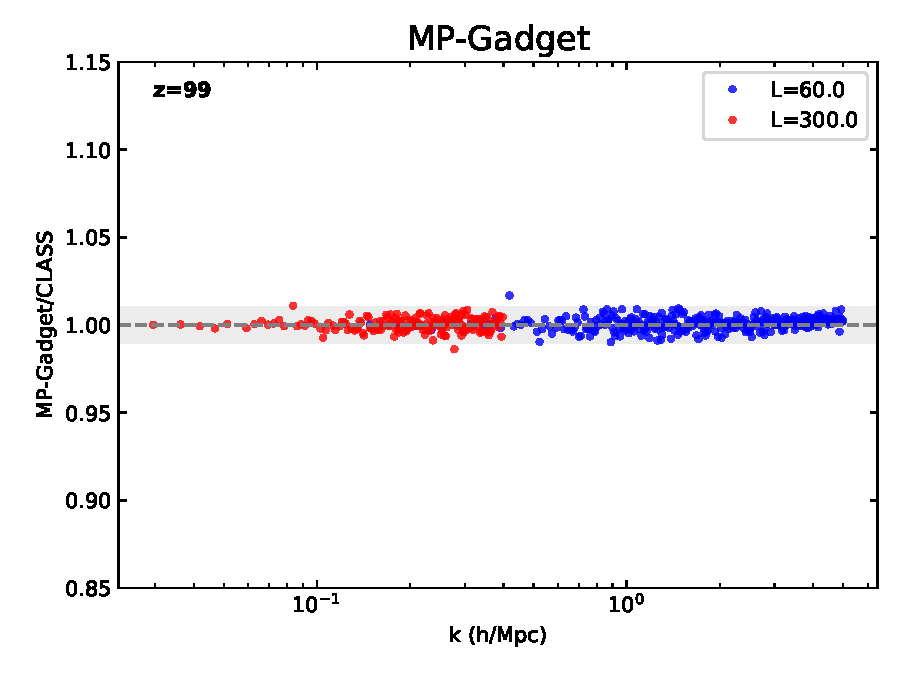
\includegraphics[scale=0.40]{MPGadget/1pc_DMONLY_MPGadget_z99_.pdf}}
	\subfigure{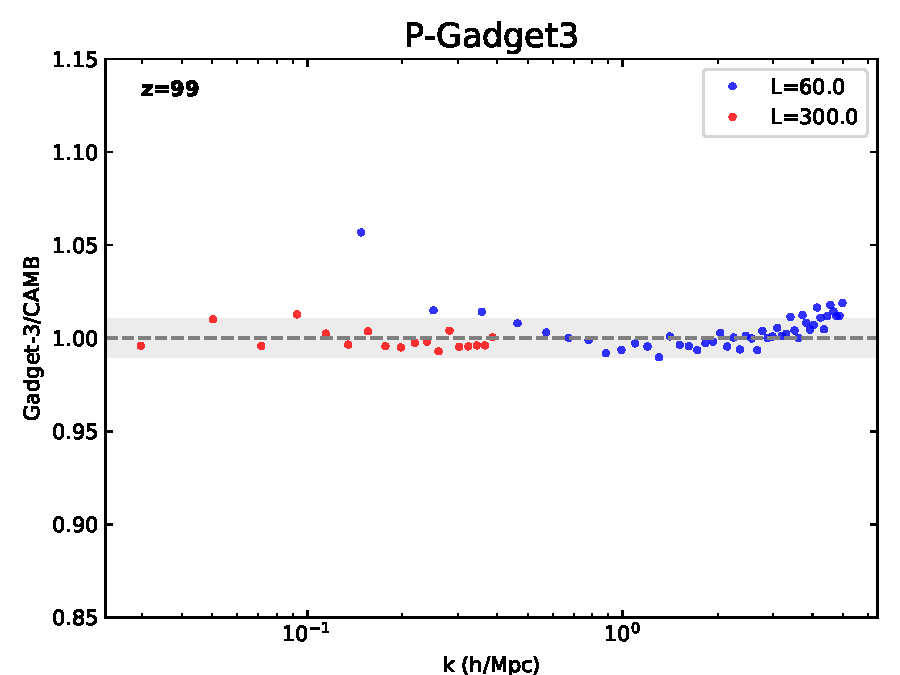
\includegraphics[scale=0.40]{Gadget3/2boxG3_1pc_1fluids_z99.pdf}}
	\subfigure{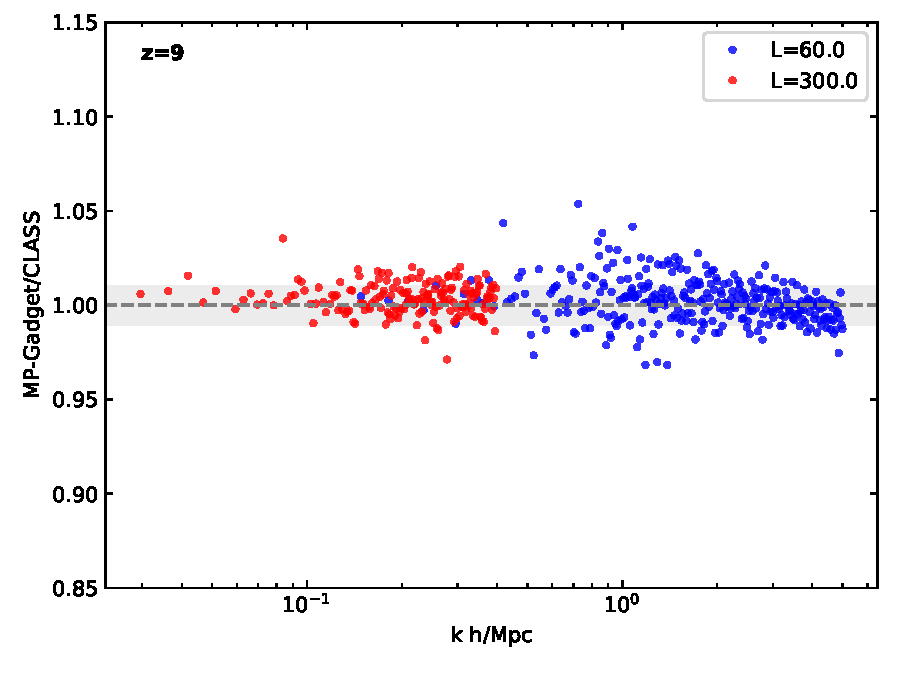
\includegraphics[scale=0.40]{MPGadget/1pc_DMONLY_MPGadget_z9_.pdf}}
	\subfigure{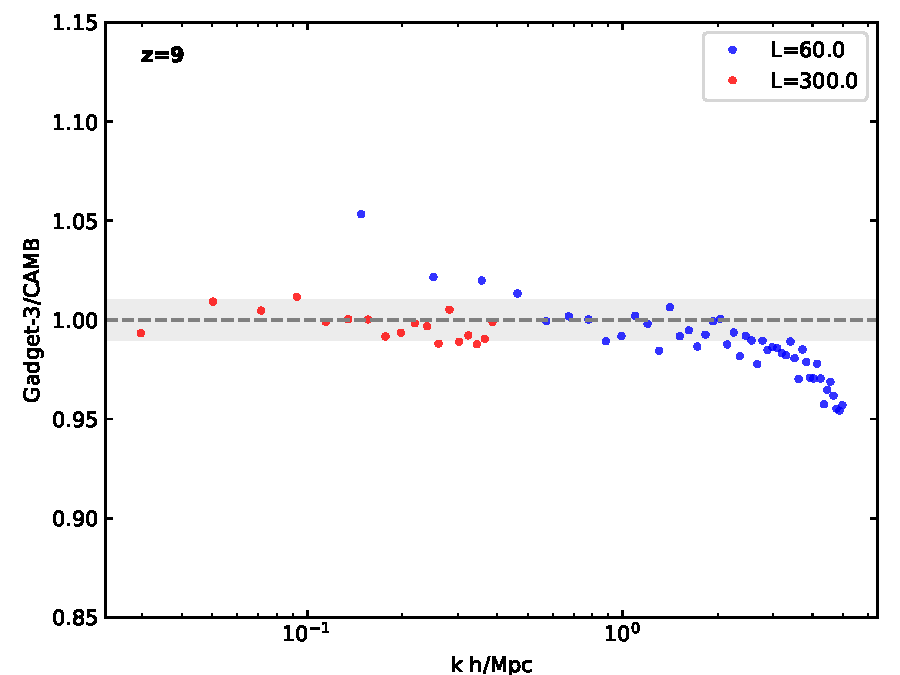
\includegraphics[scale=0.40]{Gadget3/2boxG3_1pc_1fluids_z9.pdf}}
	\subfigure{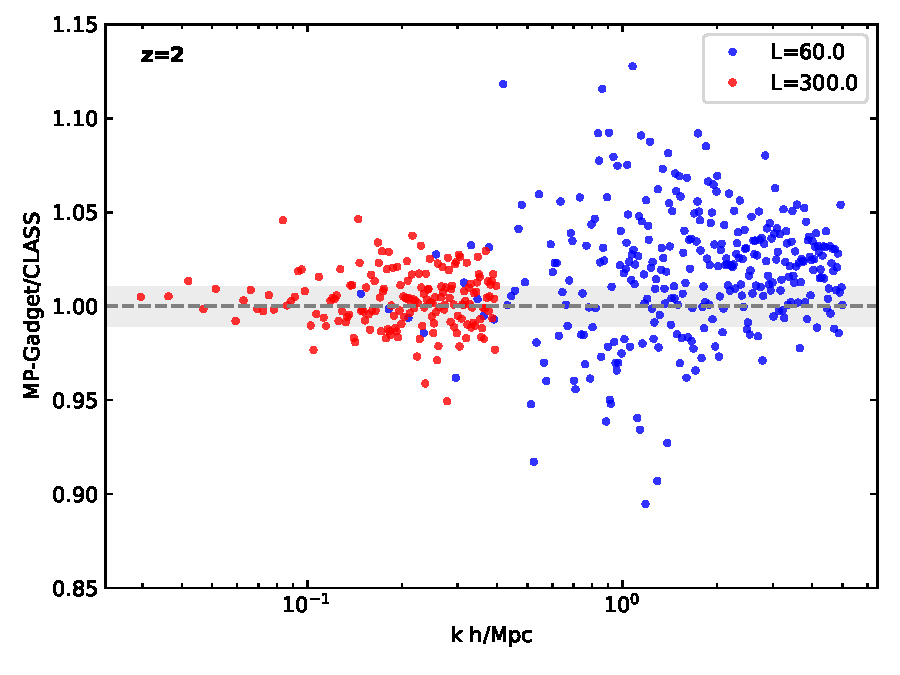
\includegraphics[scale=0.40]{MPGadget/1pc_DMONLY_MPGadget_z2_.pdf}}
	\subfigure{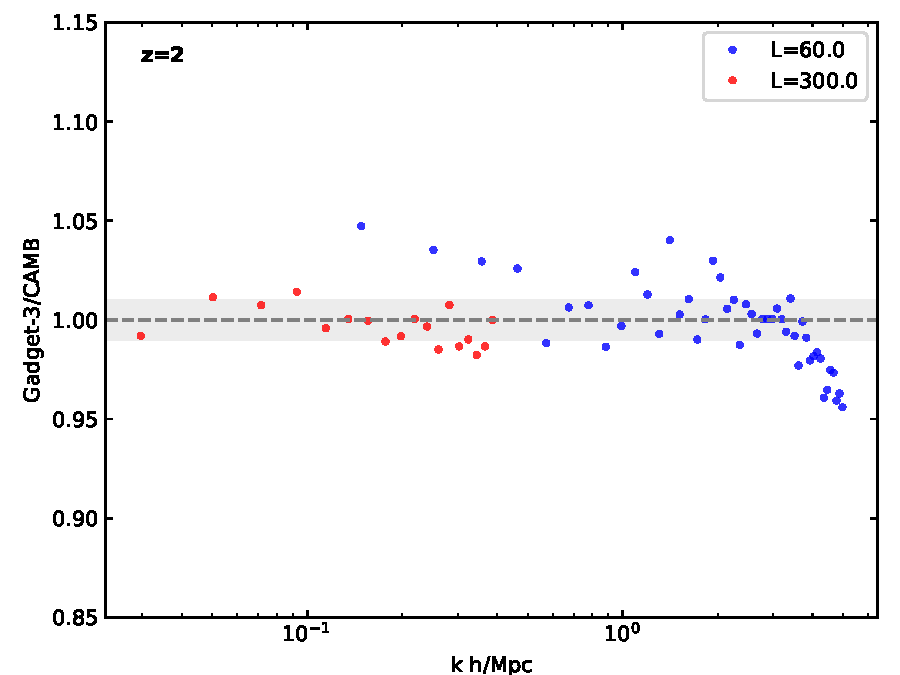
\includegraphics[scale=0.40]{Gadget3/2boxG3_1pc_1fluids_z2.pdf}}
	\caption{Left: MP-Gadget, $512^3$ particle DM-only sim. Right: P-Gadget3, $256^3$ particle DM-only
sim. Shaded area represents the $1\%$ error region, and we show results for $L=300h/\mathrm{Mpc}$ and
$L=60h/\mathrm{Mpc}$ boxes to cover a larger range of $k$ values. There is some scatter in the modes, but broadly the growth is accurate and in agreement with the predictions of linear theory. We note that in the P-Gadget3 simulations, there is an excess of power in the low-$k$ modes of the small box. We think this is a binning issue caused by the fact that the $k$-bins in this power spectrum estimator are large, and around the BAO scale will have significant gradient across them.}
\end{figure}

\clearpage


\subsection{Power spectra ratios for two particle species}

%\begin{center}
% {\large \textbf{Power spectra ratios for two particle species}}
%\end{center}

\begin{figure}[h]
	\centering
	\subfigure{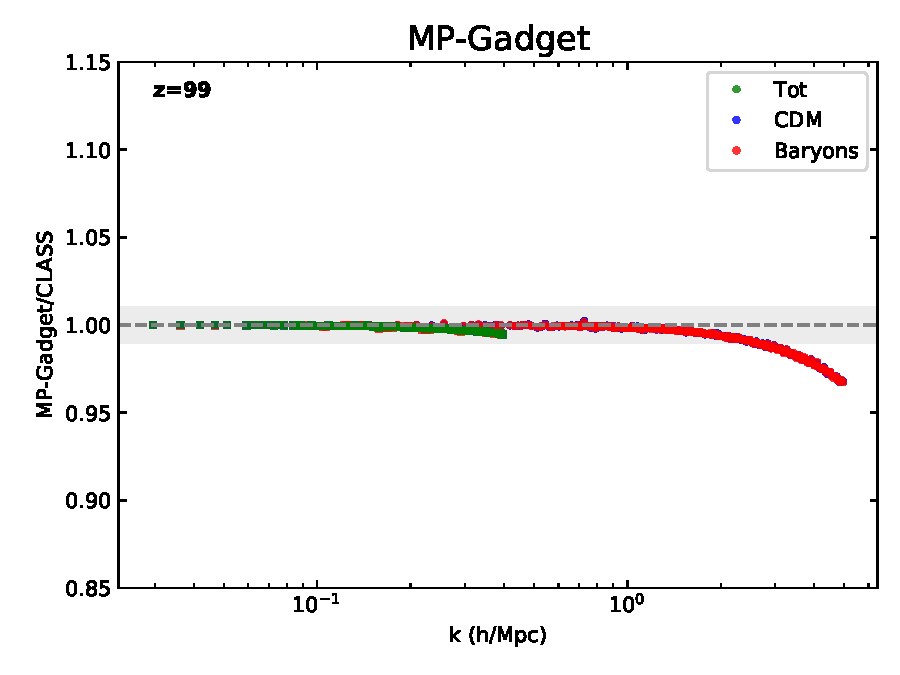
\includegraphics[scale=0.40]{MPGadget/1pc_2FLUIDS_MPGadget_z99_.pdf}}
	\subfigure{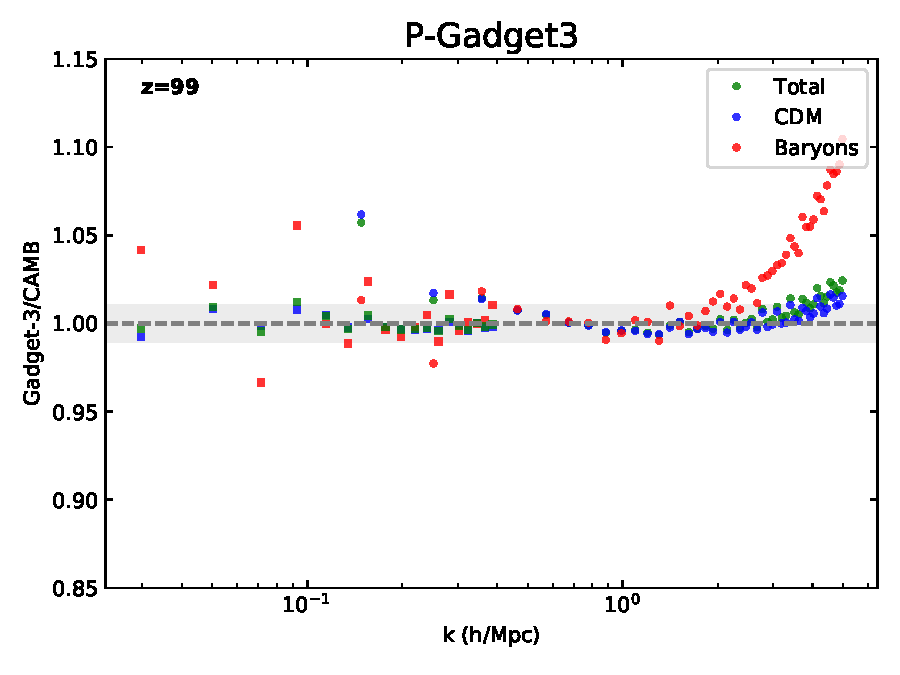
\includegraphics[scale=0.40]{Gadget3/2boxG3_1pc_2fluids_z99.pdf}}
	\subfigure{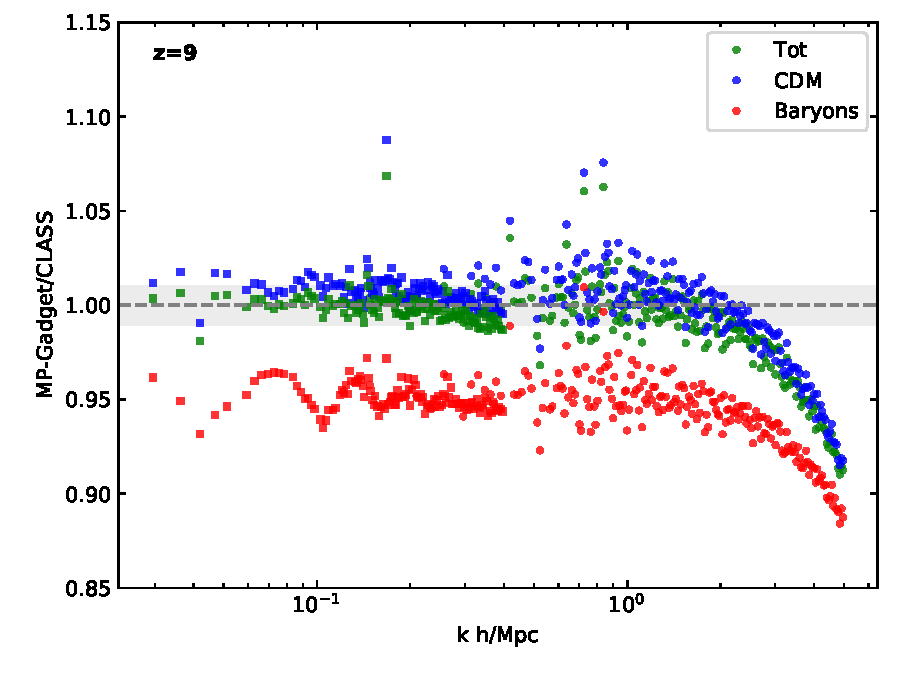
\includegraphics[scale=0.40]{MPGadget/1pc_2FLUIDS_MPGadget_z9_.pdf}}
	\subfigure{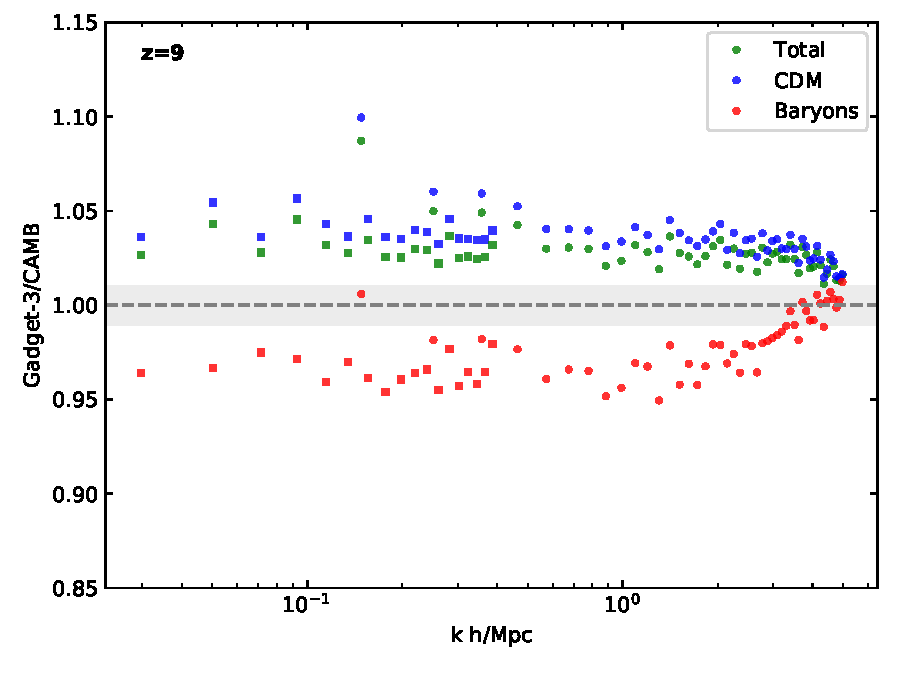
\includegraphics[scale=0.40]{Gadget3/2boxG3_1pc_2fluids_z9.pdf}}
	\subfigure{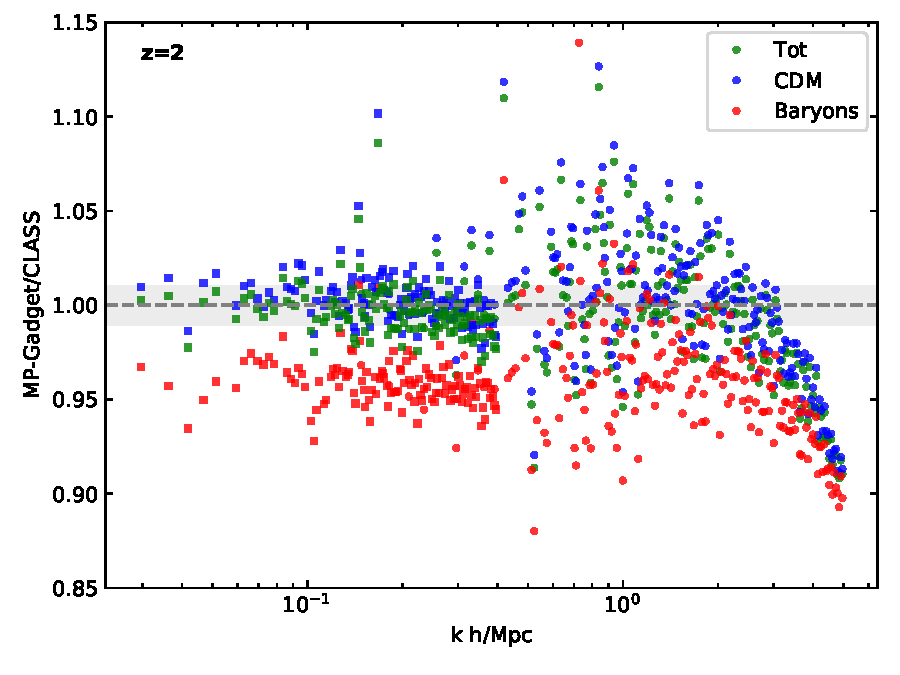
\includegraphics[scale=0.40]{MPGadget/1pc_2FLUIDS_MPGadget_z2_.pdf}}
	\subfigure{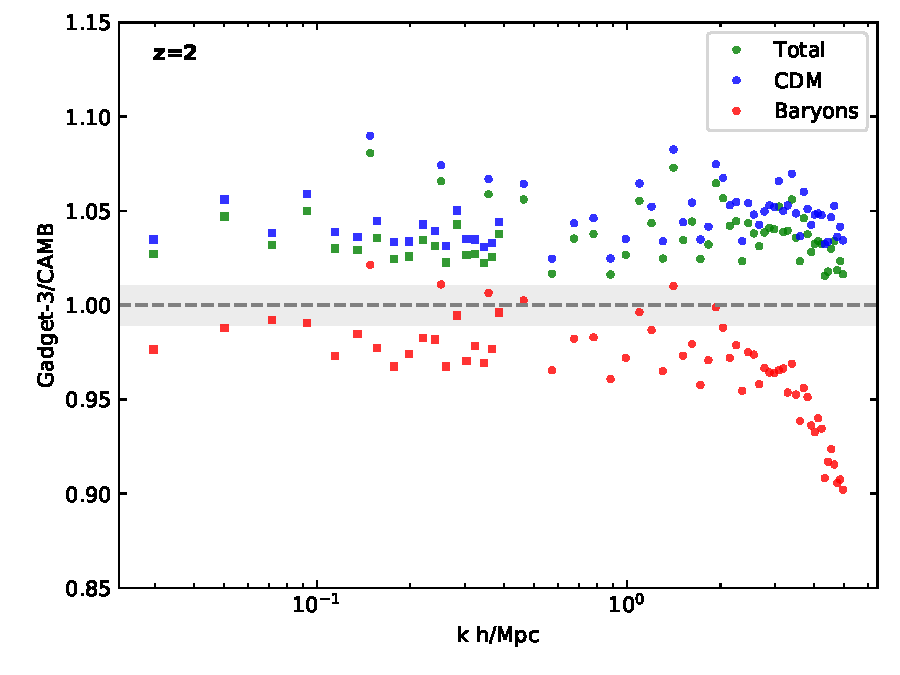
\includegraphics[scale=0.40]{Gadget3/2boxG3_1pc_2fluids_z2.pdf}}
	\caption{The same test as in the previous figure but this time with both DM and baryon particles, with MP-Gadget on left and
P-Gadget3 on the right. Again we have used two box sizes, with $L=300h/\mathrm{Mpc}$ shown in squares,
and $L=60h/\mathrm{Mpc}$ in circles. We plot the power in each simulation divided by the linear theory
prediction for that individual species. For the case of multiple species, we see that the baryon power doesn't catch up to the CDM power as quickly as linear theory predicts. In MP-Gadget, the error in the baryon and CDM power approximately cancels out to give an accurate total matter, however in P-Gadget3, even the total growth is inaccurate with multiple species.
\pvm{Why does Fig. \ref{fig:treenotree} have so much less scatter?}}
\CP{This is because the noise in each mode is the same in the CDM and baryons, so the
ratio of the two is smooth}
\end{figure}

\clearpage

\subsection{Effect of Tree in multiple species simulations}


%\begin{center}
% {\large \textbf{Effect of Tree in multiple species simulations}}
%\end{center}
\begin{figure}[h]
	\centering
	\subfigure{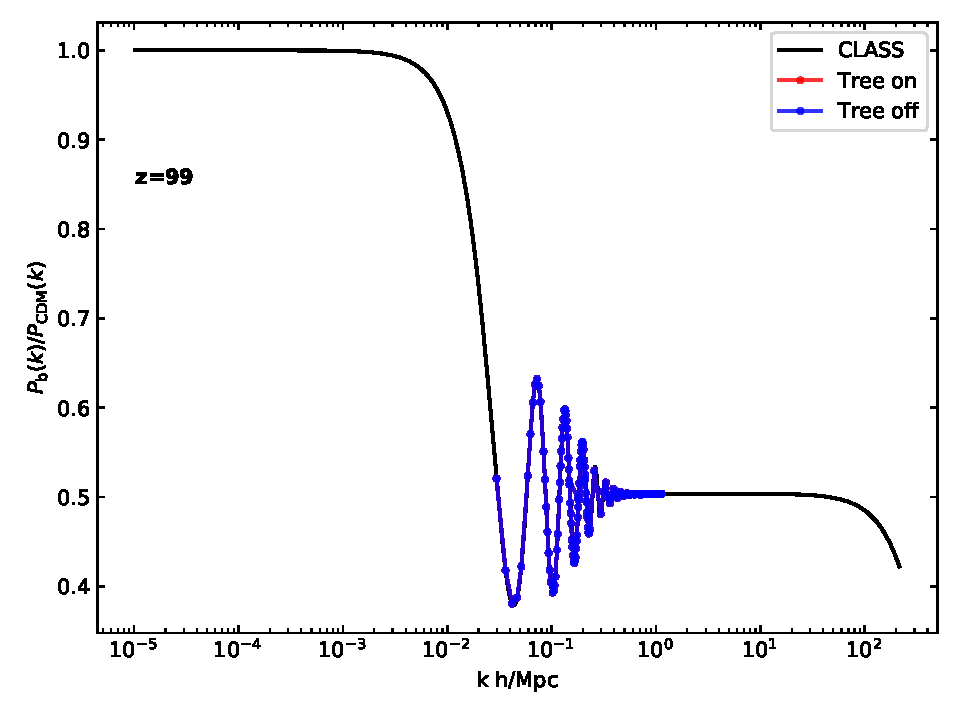
\includegraphics[scale=0.45]{MPGadget/bycdm_MPGadget_z99_.pdf}}
	\subfigure{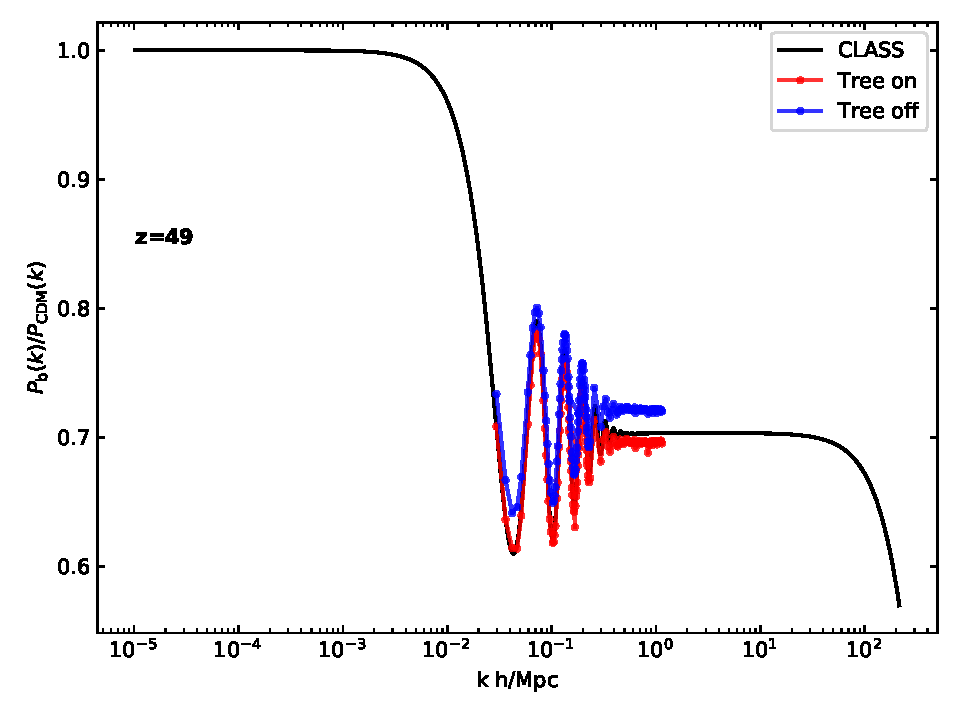
\includegraphics[scale=0.45]{MPGadget/bycdm_MPGadget_z49_.pdf}}
	\subfigure{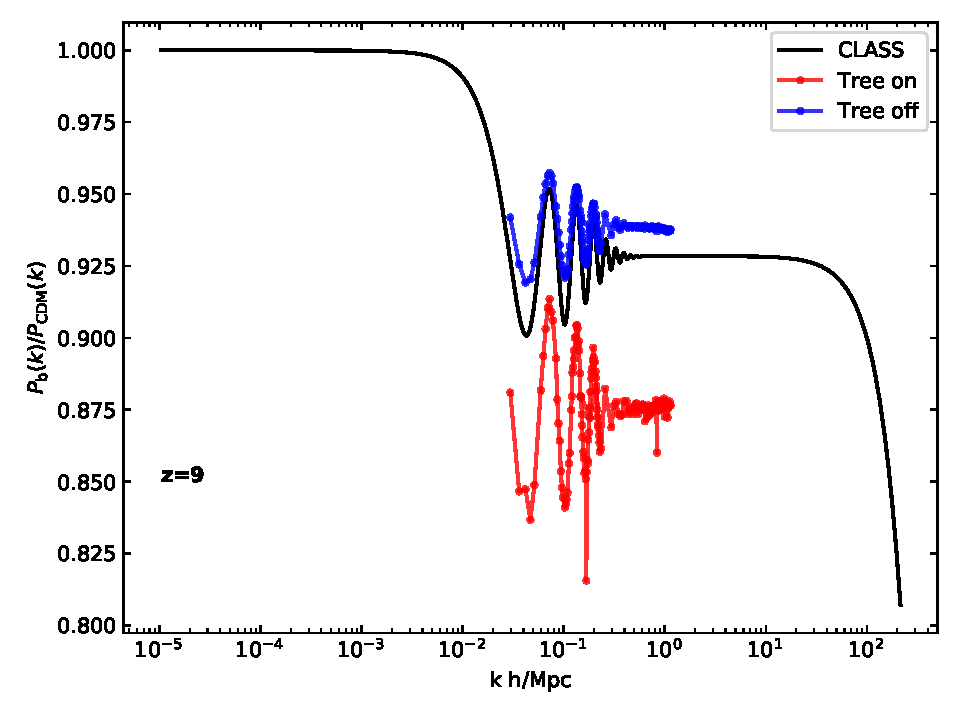
\includegraphics[scale=0.45]{MPGadget/bycdm_MPGadget_z9_.pdf}}	
	\subfigure{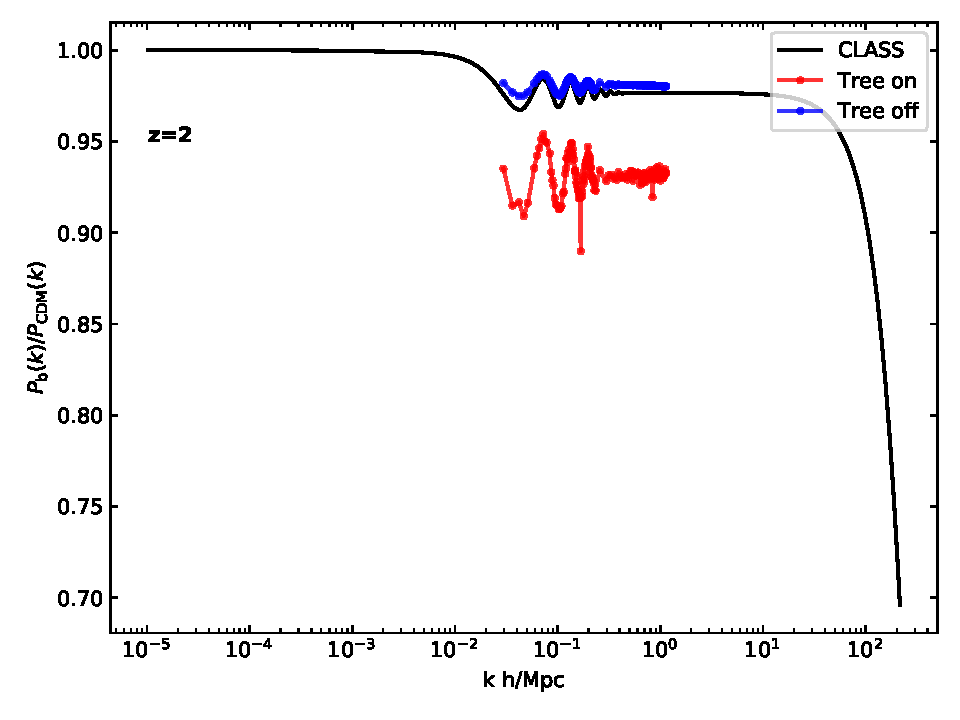
\includegraphics[scale=0.45]{MPGadget/bycdm_MPGadget_z2_.pdf}}
	\caption{Effect of Tree on the ratios of the baryon and CDM power in MP-Gadget simulations. Turning on the Tree has a significant effect on the relative power in the two particle species, even on large scales.
\label{fig:treenotree}}
\end{figure}

\clearpage

\subsection{Adaptive softenings}
\begin{figure}[h]
	\centering
	\subfigure{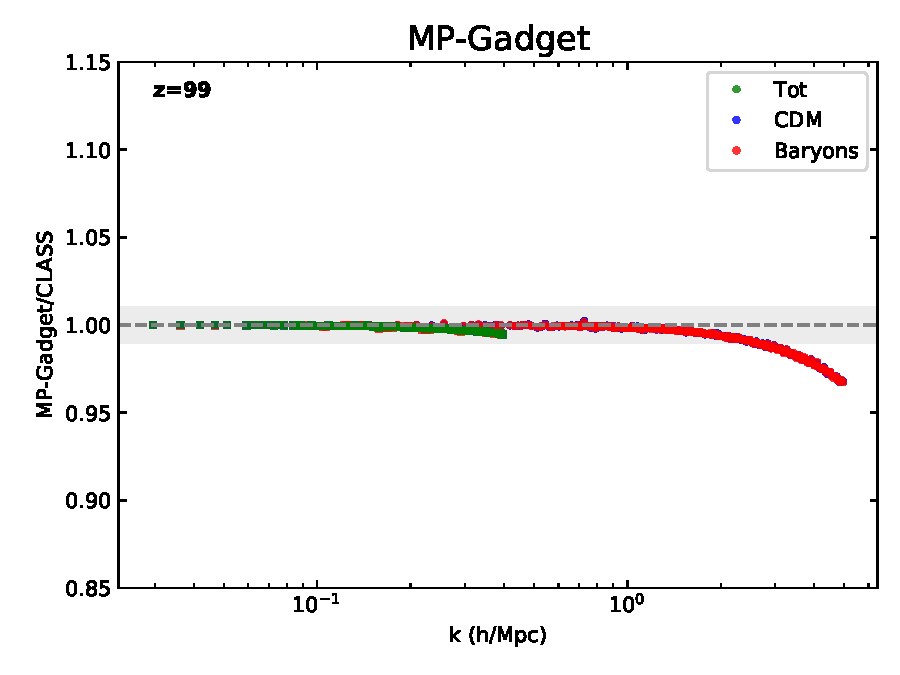
\includegraphics[scale=0.34]{MPGadget/1pc_2FLUIDS_MPGadget_z99_.pdf}}
	\subfigure{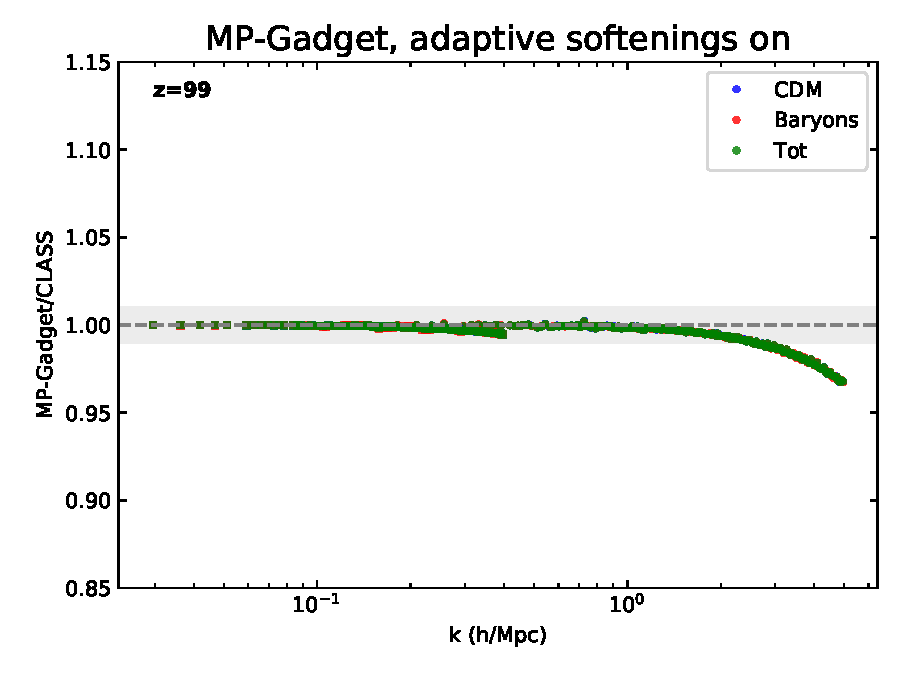
\includegraphics[scale=0.34]{MPGadget/Adaptive_1pc_2FLUIDS_MPGadget_z99_.pdf}}
	\subfigure{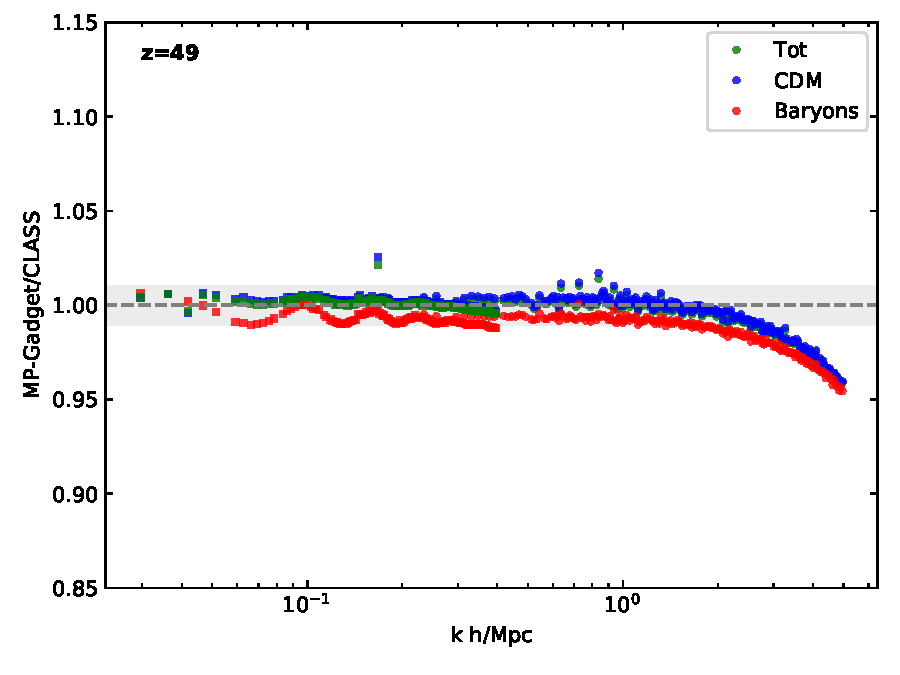
\includegraphics[scale=0.34]{MPGadget/1pc_2FLUIDS_MPGadget_z49_.pdf}}
	\subfigure{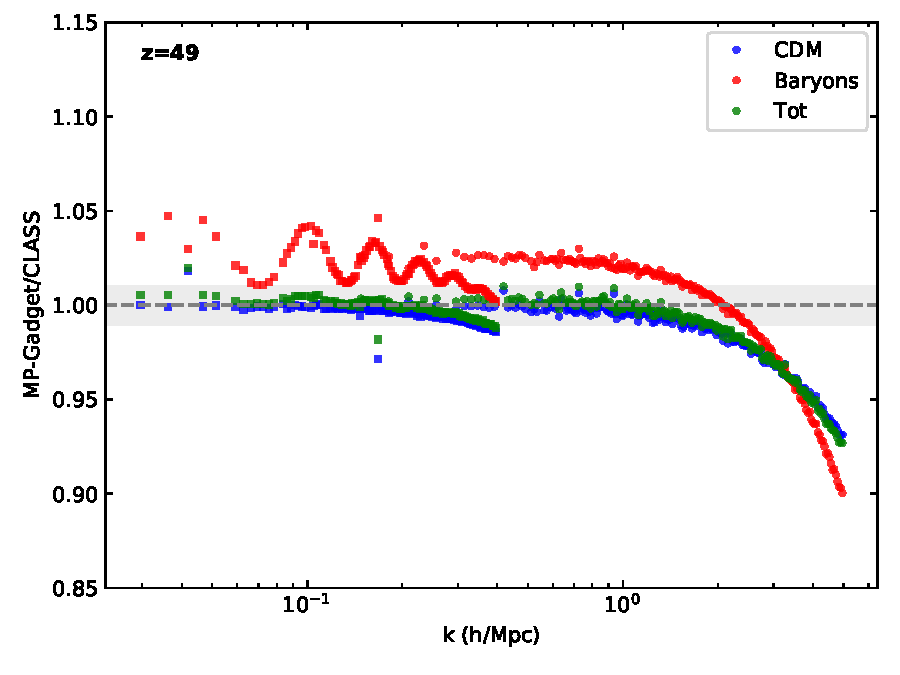
\includegraphics[scale=0.34]{MPGadget/Adaptive_1pc_2FLUIDS_MPGadget_z49_.pdf}}
	\subfigure{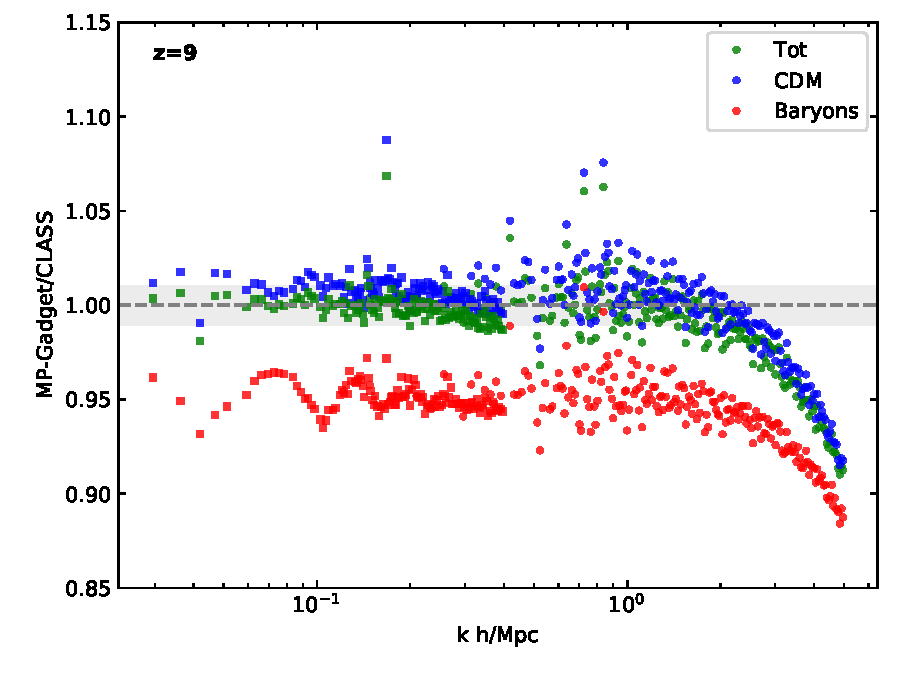
\includegraphics[scale=0.34]{MPGadget/1pc_2FLUIDS_MPGadget_z9_.pdf}}
	\subfigure{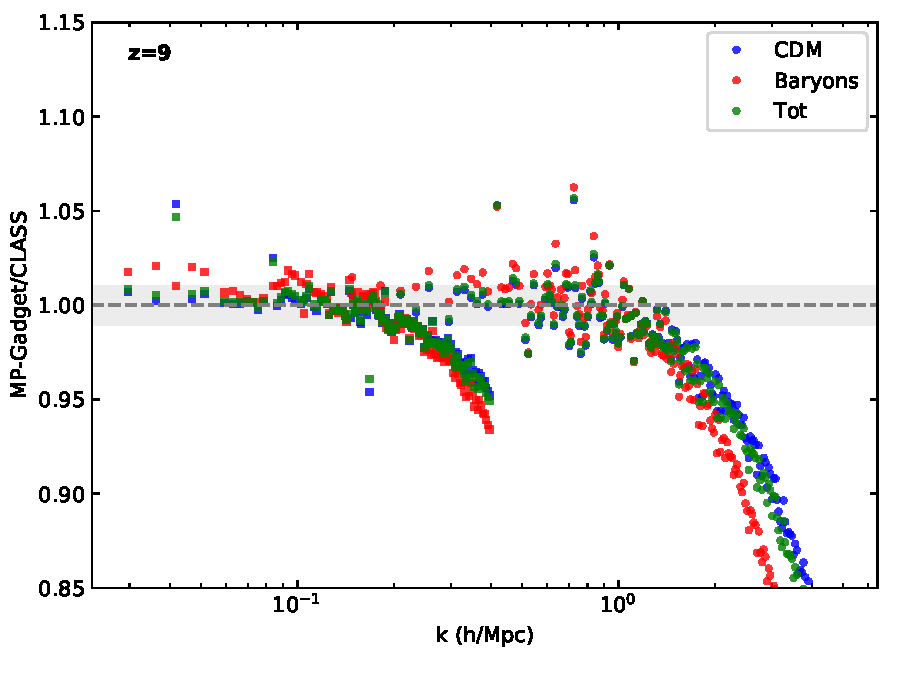
\includegraphics[scale=0.34]{MPGadget/Adaptive_1pc_2FLUIDS_MPGadget_z9_.pdf}}
	\subfigure{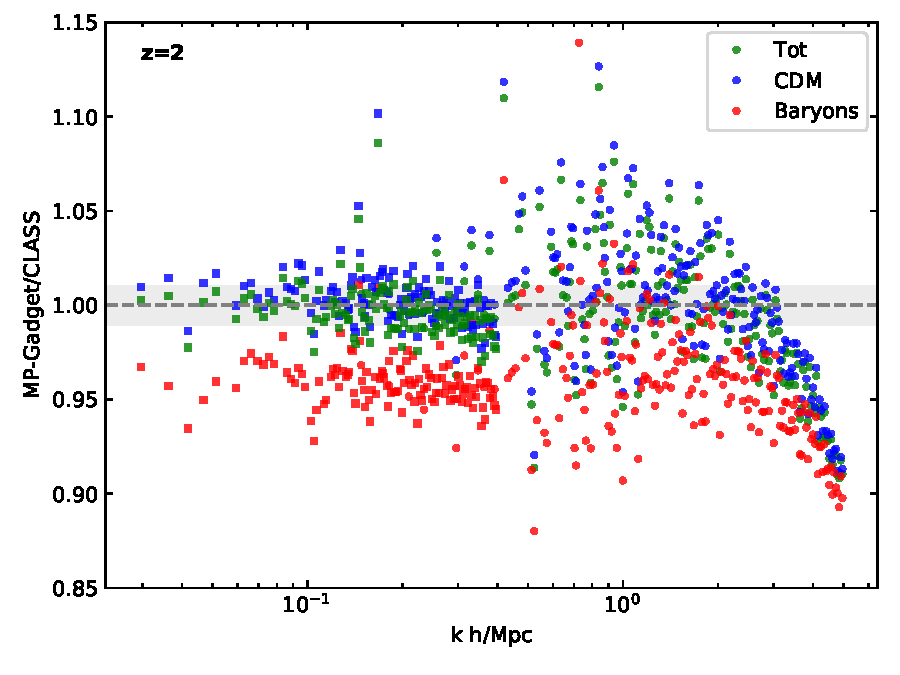
\includegraphics[scale=0.34]{MPGadget/1pc_2FLUIDS_MPGadget_z2_.pdf}}
	\subfigure{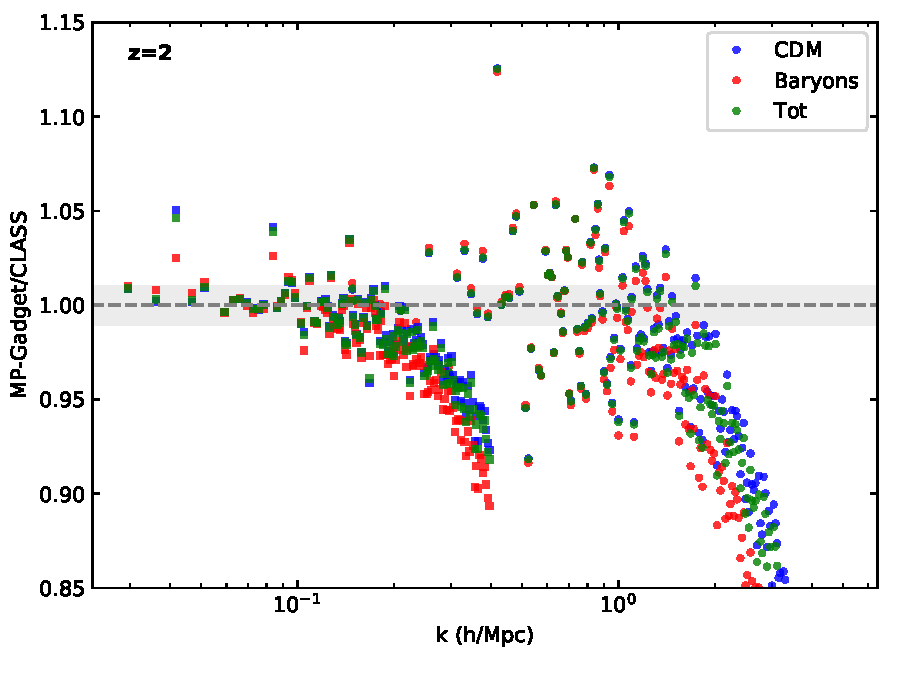
\includegraphics[scale=0.34]{MPGadget/Adaptive_1pc_2FLUIDS_MPGadget_z2_.pdf}}
	\caption{Comparison of the effect of adaptive softening on $1\%$ growth tests. We note that the adaptive softening improves the deficiency in baryon power, however at the cost of a suppression of power at higher $k$ as a result of force smoothing on small scales. In agreement with Fig. 1 of ref \cite{Angulo2013}, we find that the effect of adaptive softenings is very similar to simply turning off the Tree.}
\end{figure}
\clearpage
\subsection{Oversampling CDM particles}
\begin{figure}[h]
	\centering
	\subfigure{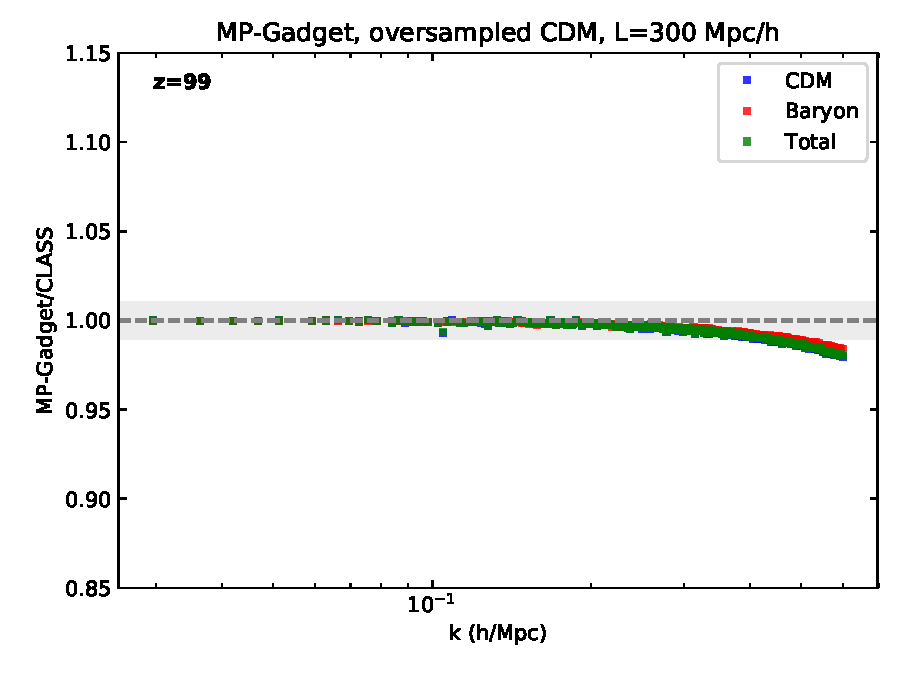
\includegraphics[scale=0.45]{MPGadget/oversample_MPGadget_z99_.pdf}}
	\subfigure{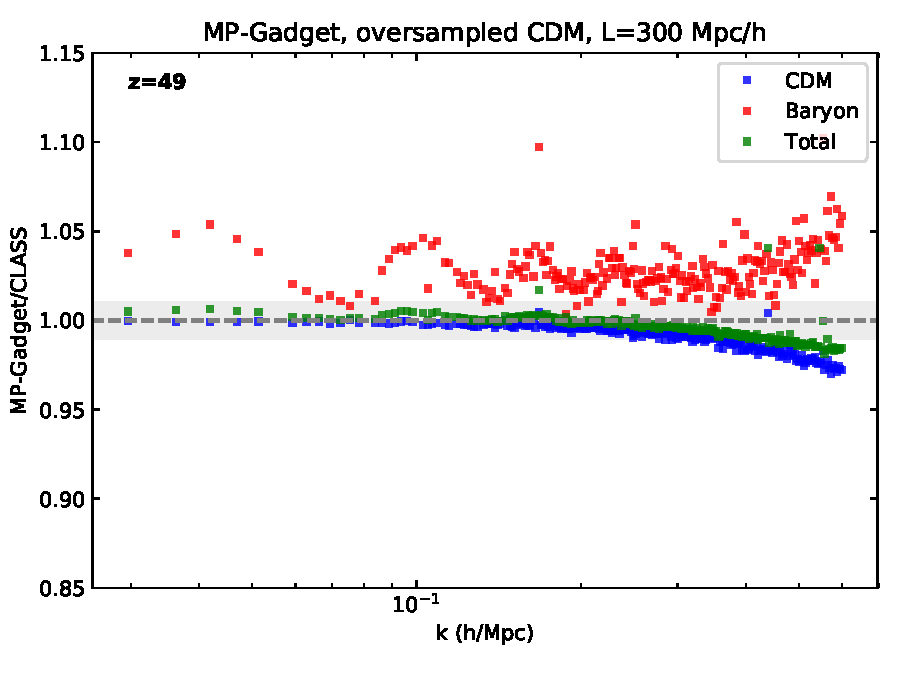
\includegraphics[scale=0.45]{MPGadget/oversample_MPGadget_z49_.pdf}}
	\subfigure{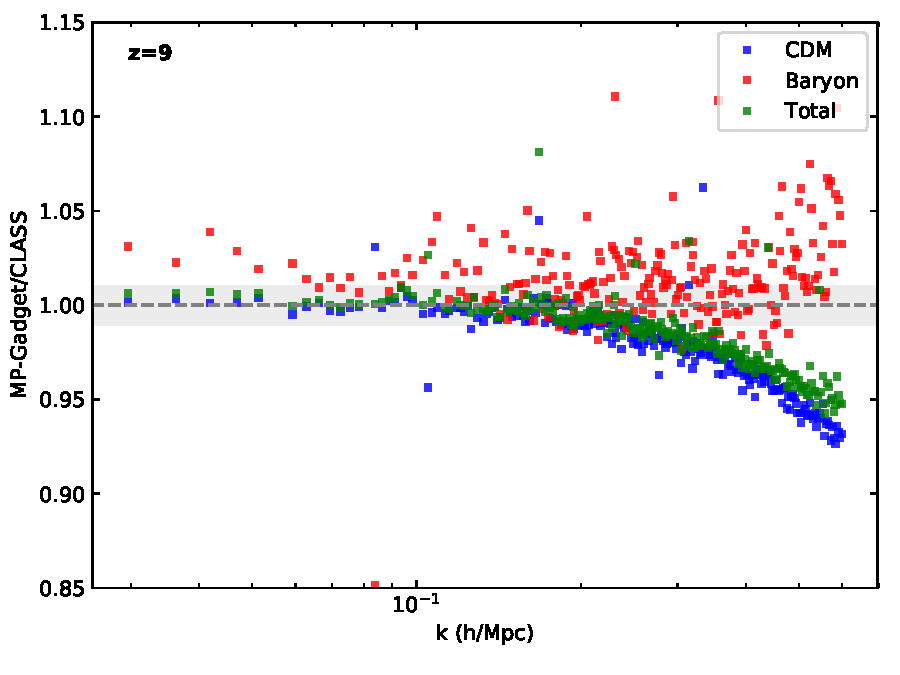
\includegraphics[scale=0.45]{MPGadget/oversample_MPGadget_z9_.pdf}}	
	\subfigure{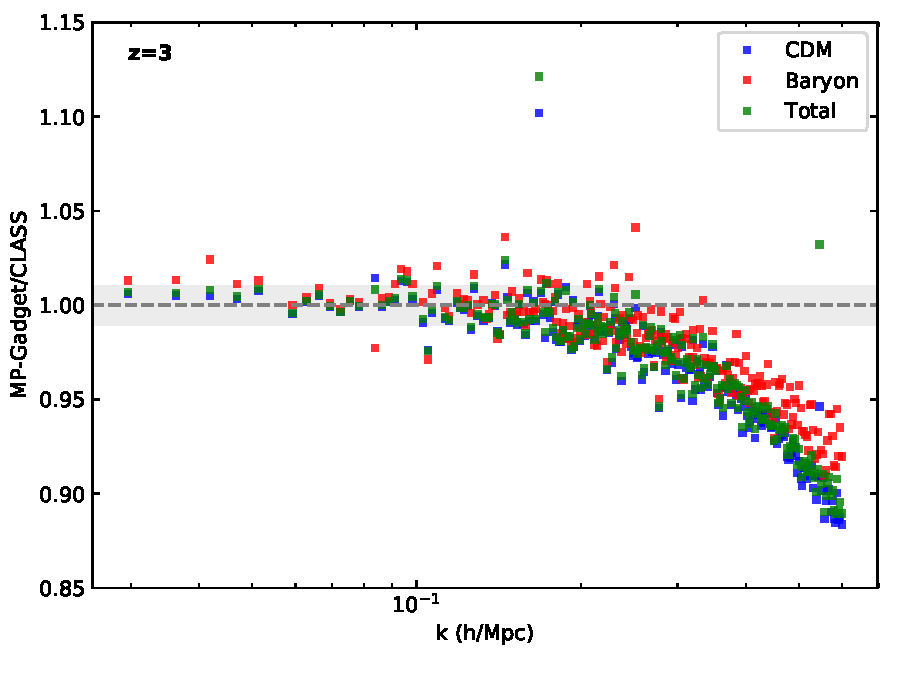
\includegraphics[scale=0.45]{MPGadget/oversample_MPGadget_z3_.pdf}}
	\caption{Effect of increasing the number of CDM particles to ensure that they have the same mass as baryon particles. This result significantly improves the accuracy of the power in each species at low $z$, but at the cost of a factor of 6 increase in CPU time, and the high $z$ growth is still not accurate.}
\end{figure}
\clearpage
\subsection{GLASS initial conditions}

\begin{figure}[h]
        \centering
        \subfigure{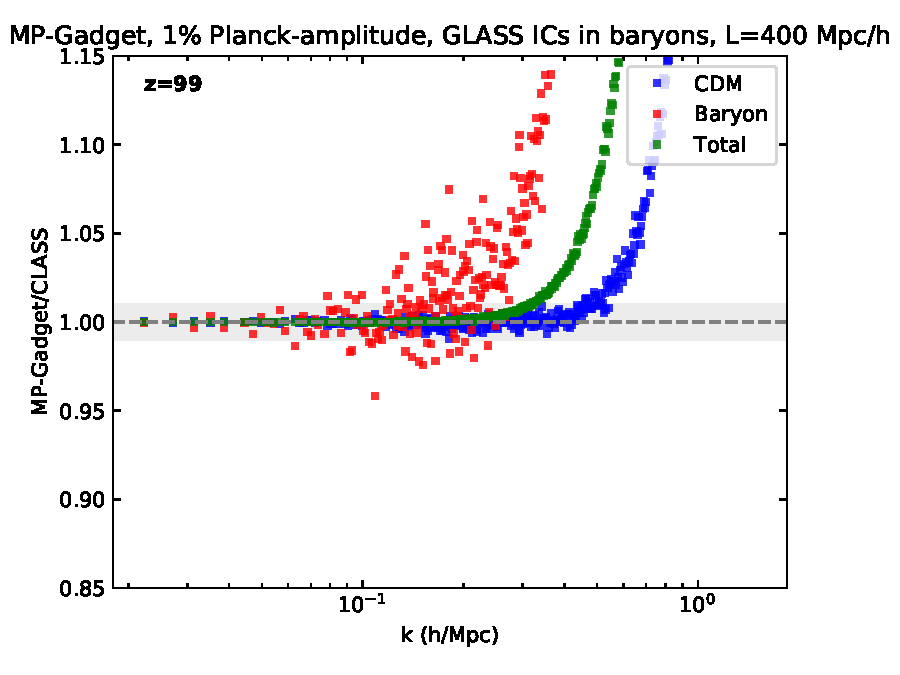
\includegraphics[scale=0.45]{MPGadget/GlassOn_lowamp_z99.pdf}}
        \subfigure{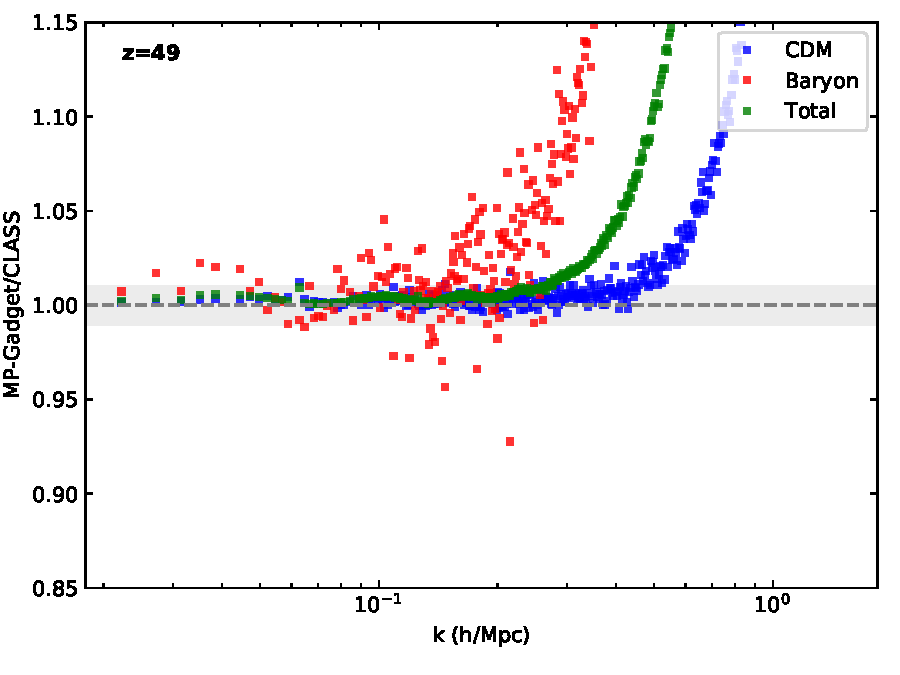
\includegraphics[scale=0.45]{MPGadget/GlassOn_lowamp_z49.pdf}}
        \subfigure{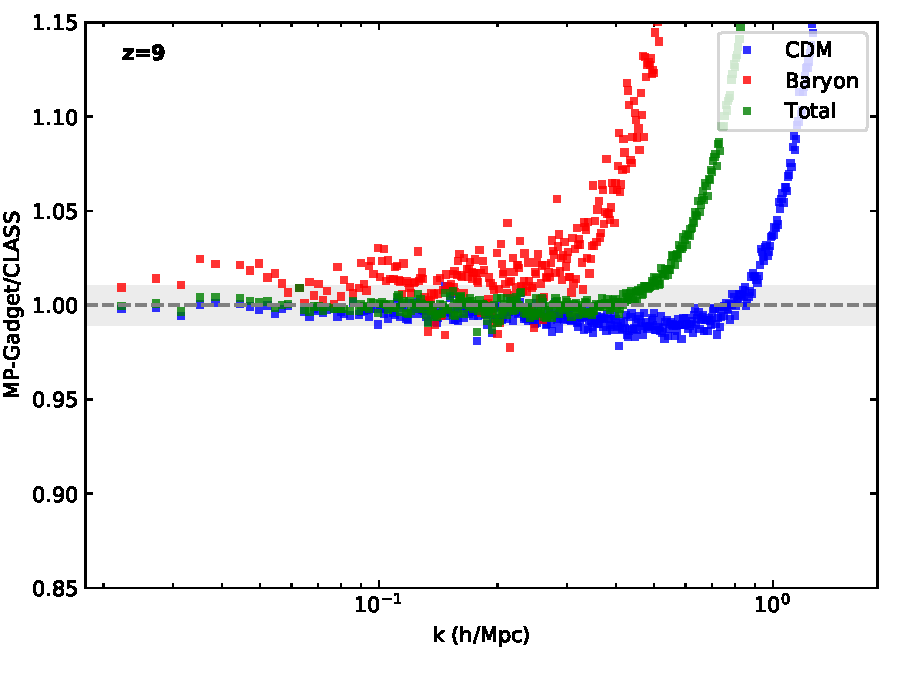
\includegraphics[scale=0.45]{MPGadget/GlassOn_lowamp_z9.pdf}}
        \subfigure{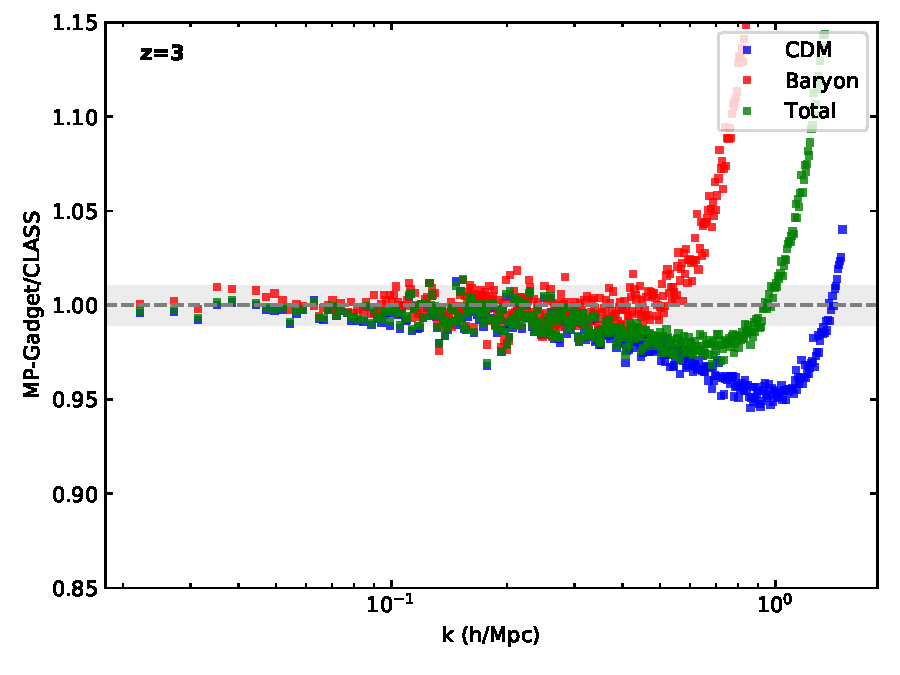
\includegraphics[scale=0.45]{MPGadget/GlassOn_lowamp_z3.pdf}}
        \caption{Effect of using GLASS ICs in the baryons in simulations in the reduced
amplitude cosmology. Here the CDM particles are
seeded using the standard grid ICs, but the baryons are initialised using a GLASS file
in order to break the regularity of the staggered grid structure. The spike in baryon
power at high $k$ is the result of a $\propto k^4$ noise that comes from the GLASS file.
The disparity on large scales between the simulation power and linear theory is reduced
significantly at $z=2$, with a slight excess in baryon power at $z=9$. Not sure why there is
also a spike in CDM power on small scales.}
\end{figure}
\clearpage
\begin{figure}[h]
        \centering
        \subfigure{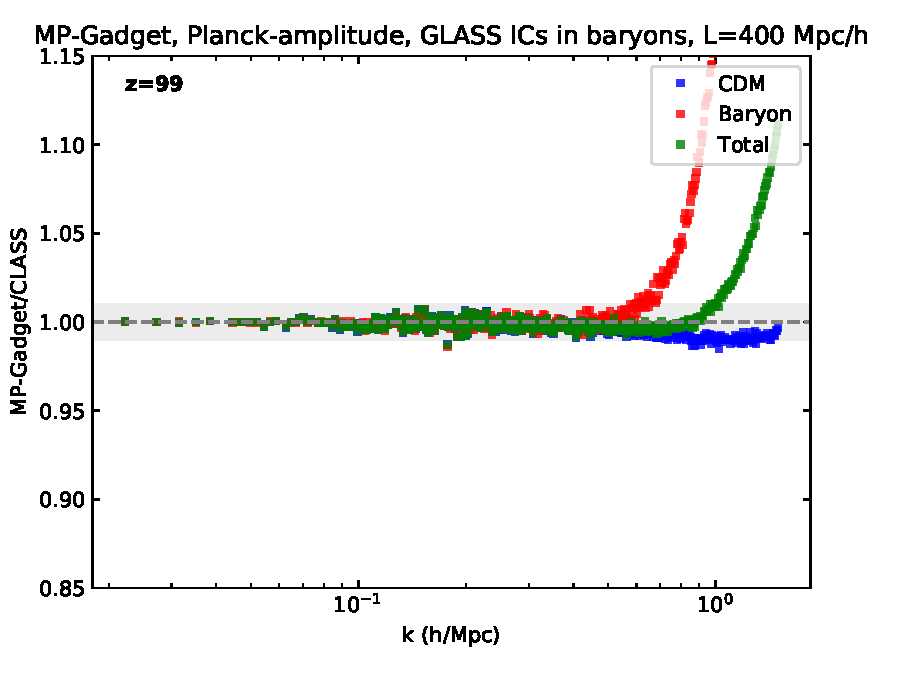
\includegraphics[scale=0.45]{MPGadget/GlassOn_fullamp_z99.pdf}}
        \subfigure{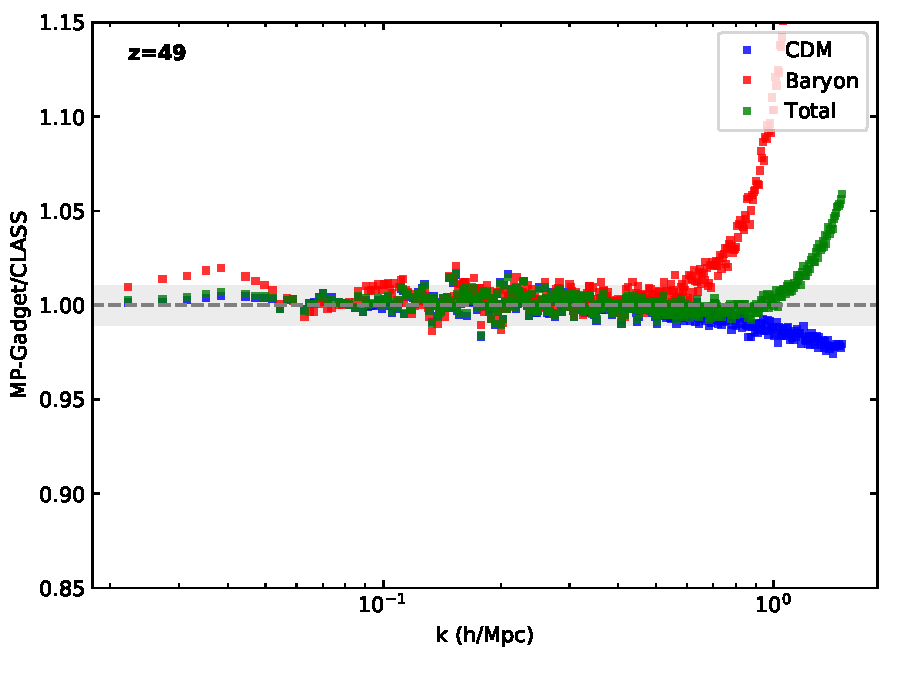
\includegraphics[scale=0.45]{MPGadget/GlassOn_fullamp_z49.pdf}}
        \subfigure{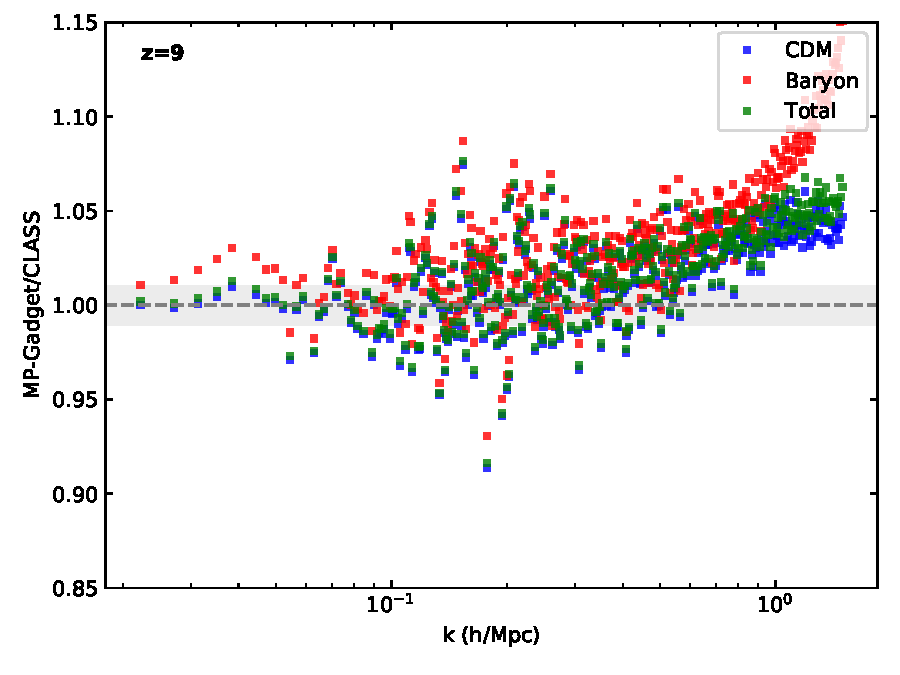
\includegraphics[scale=0.45]{MPGadget/GlassOn_fullamp_z9.pdf}}
        \subfigure{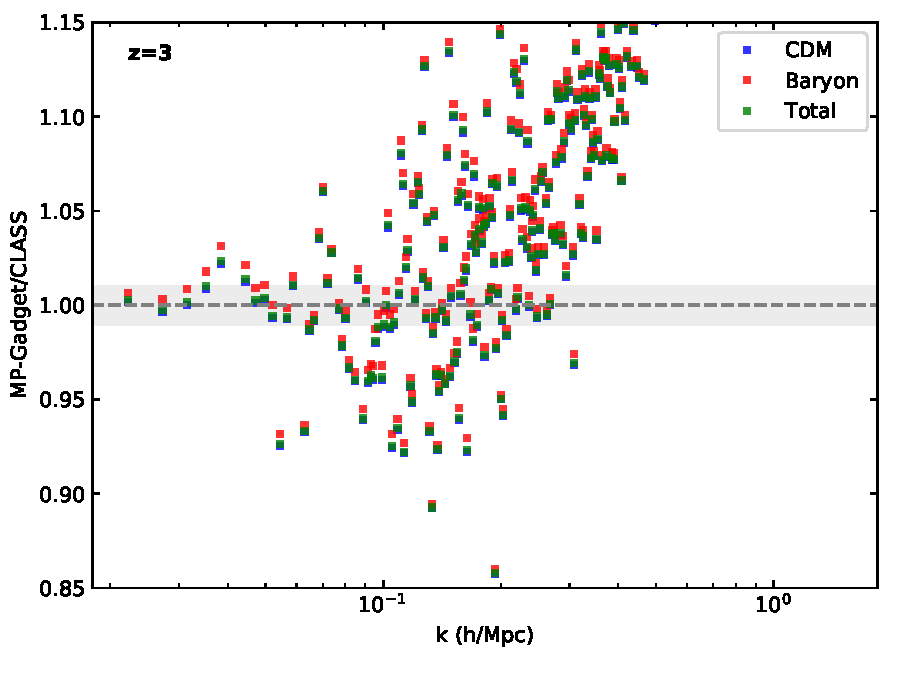
\includegraphics[scale=0.45]{MPGadget/GlassOn_fullamp_z3.pdf}}
        \caption{The same test as previous, except run with full amplitude. The notable
differences are that the GLASS noise is less prominent than in the low amplitude test,
and the CDM power doesn't spike at high $k$.}
\end{figure}

\clearpage
\subsection{Summary}
We present a set of simulations aimed at testing the accuracy of the growth of structure in Gadget cosmology simulations by reducing their non-linearities at low redshift and comparing the power spectra with that predicted by linear theory. We find good agreement in the case of simulations with only one particle type, but find that the simulations do not produce correct clustering statistics for each individual particle type in the case of simulations involving both CDM and baryon particles seeded with different initial power spectra. The Tree algorithm was shown to have a significant effect on the relative power in the two species, even on large scales, although in the opposite direction to that found in \cite{Angulo2013}. We note here that if you swap the short range force from the Tree to a direct summation solver, this does not solve the problem. There is some disagreement on small scales on the order of $5\%$ when comparing the short range Tree with direct summation, however the large scale power is unaffected meaning this issue is not a result of inaccuracy of the Tree algorithm. Finally we showed that adaptive softening can improve the relative power issue on large scales, but at the expense of suppressing power on small scales, which is a similar effect to turning the Tree off. So currently, the trade off appears to be between having accurate total matter on all scales but with low baryon power, or accurate power in both CDM and baryons on large scales but with low power in all species on small scales.
\pvm{You do say here that you checked this... but you don't sound so 
confident in conversations. I'd like to see at least a factor 2 bigger
$r_s$.}
\CP{Yes this was a mistake, I added this after making small changes to the transition
scale before we realised that the code couldn't actually handle this.}

\subsection{Appendix/Questions from Pat}

\pvm{It would be good to see if the offset depends on the initial power 
(displacement) level, e.g., 1\% of Planck vs. 10\%.
}
\CP{I have checked this, and its independent of the amplitdue of the initial power,
i.e. if you use large boxes and 100\% Planck amplitude, you still get the same offset.
Also the same for 10\%}

\pvm{You could check for post-reionization Compton drag effects in CAMB by
comparing transfer functions with significantly different optical depth
values... i.e., default expectation would be that this effect would be tiny,
but... I'm too lazy to figure out from Chen paper what they're saying the
size of effect is.} 

\pvm{To be clear, when you say ``CLASS" in the denominator, you mean the
similarly binned spectrum with mode amplitudes computed at this
redshift using the same IC and CLASS transfer functions?
I'm asking because it seems like that
should take out the kind of bin-offset effects you mention... and also I'm
surprised there is so much scatter... If you are using 2LPT for the IC, it
might be interesting to ``set up IC'' at $z=2$ and compare to that... even
1LPT, i.e., Zel'dovich, IC would have non-linear effects in mass power. I guess
scatter is less of an issue for your b-c comparison, but it might be a useful
sanity check to compute 2LPT prediction for $z=2$ and $z=9$. }
\CP{The modes aren't similarly binned at the moment - I am interpolating a very finely
binned CAMB power spectra so the binning in the two power spectra is different.
The ICs are also Zel'dovich, not 2LPT.}


\bibliography{refs}

\end{document}
